\documentclass{article}

\usepackage{graphicx}
\usepackage{lmodern}
\usepackage{enumitem}

\begin{document}
	\begin{titlepage}
		\fontfamily{pbk}\selectfont
		\hbox{			
			\rule{1pt}{\textheight}
			\hspace*{0.05\textwidth}
			\parbox[b]{\textwidth}{
				\Large Project Tender\\[1cm]
					
				\Huge Project: Insurance Profiling\\
				\huge Client: Retro Rabbit\\[1.5cm]					
					
				{\huge Team: HTTP\textunderscore418}
				
				\begin{itemize}[label={}, leftmargin=0pt, noitemsep]
					\Large						
					\item Christiaan Saaiman, 12059138
					\item Michael Loosen, 14017254
					\item Elizabeth Bode, 14310156
					\item LC Meyers, 14024633
				\end{itemize}
				\vspace{0.5cm}
					
				{\large Department of Computer Science, University of Pretoria\\[0.2cm]}

				\Large\today\\[0.3cm]				
									
				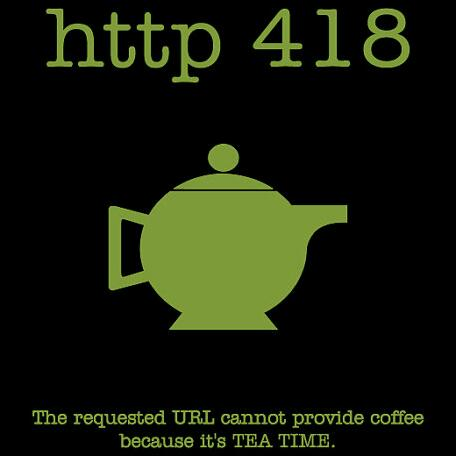
\includegraphics[scale=0.3]{../teamPic.jpg}					
			}								
		}
	\end{titlepage}
	\newpage
	\section{The Team}
	\subsection{LC Meyers}
	\begin{figure}[h]
		\centering
		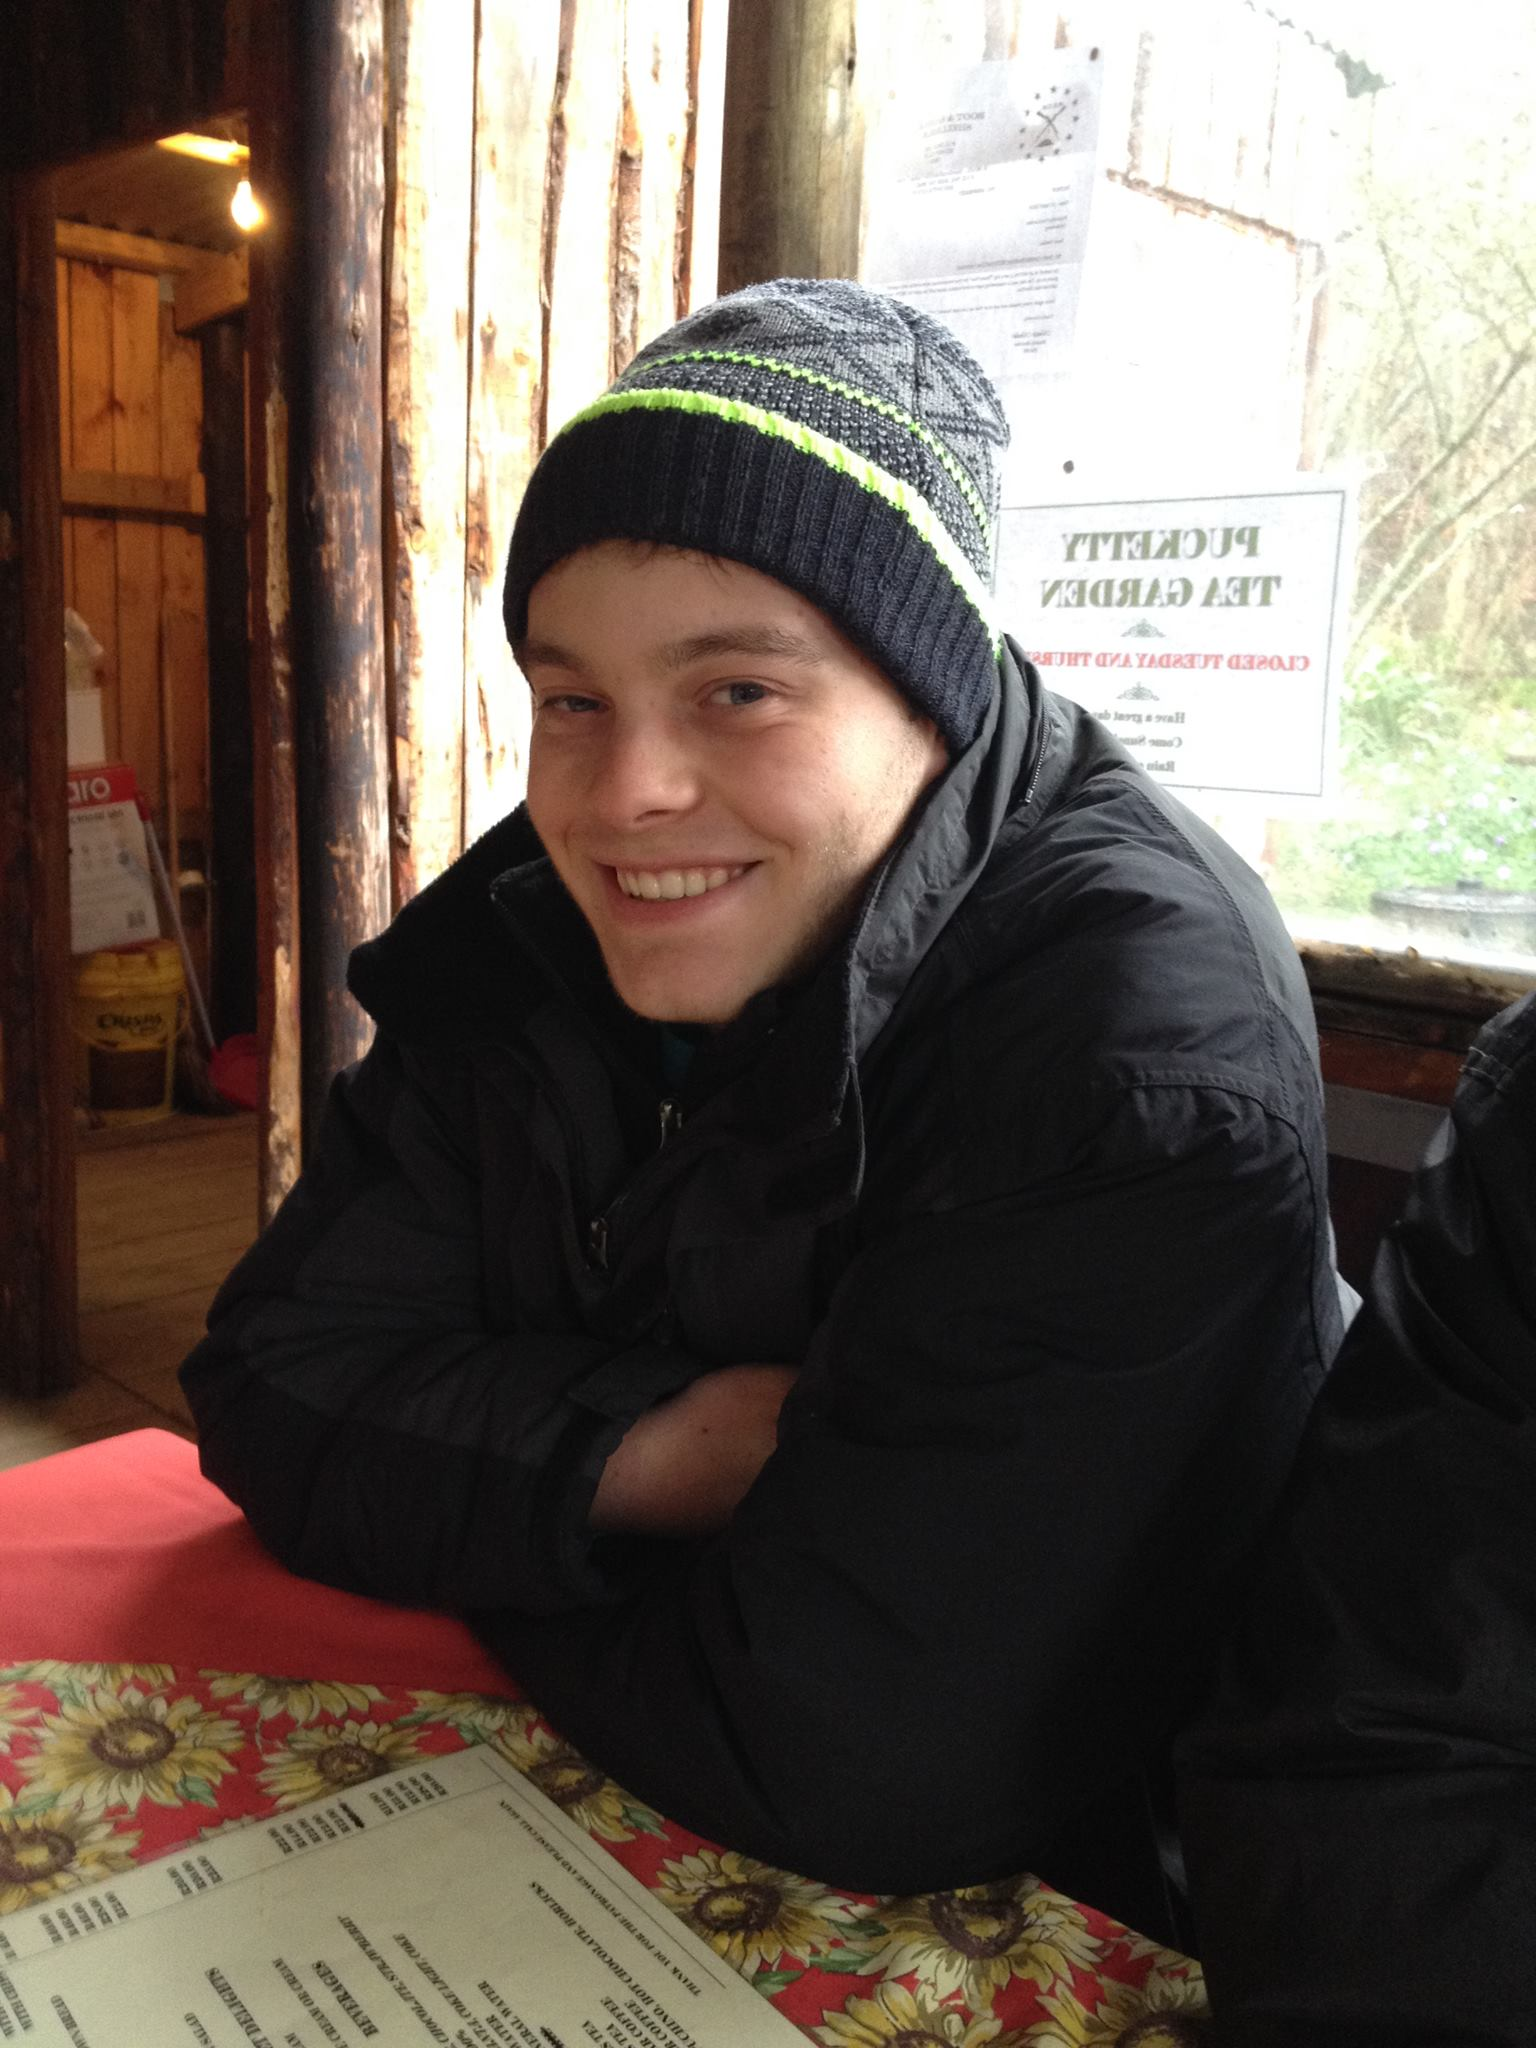
\includegraphics[height=0.3\textheight]{../charl.jpg}
	\end{figure}
	\begin{itemize}
		\item \textbf{Full name:} Lodewyk Charles Meyers
		\item \textbf{My interests:}
			\subitem Gaming
			\subitem Computers
			\subitem Music
			\subitem User experience design
			\subitem Website design
			\subitem Anything new related to technology
		\item \textbf{My technical skills:}
			\subitem Web development skills
			\subitem Database design
			\subitem Java
			\subitem C\#
		\item \textbf{Past experience that might help:}
			\subitem I collaborated on a website for a school as part of a project.
			\subitem As part of the above mentioned I had to embed a Facebook plugin into the website and have thus acquired some knowlage on how the Facebook API's work.
		\item \textbf{Non-technical strenghts:}
			\subitem I have a high amount of patience
			\subitem Hardworking
			\subitem Eager to learn new things
			\subitem Enjoy trying to solve complex problems
		\item \textbf{What makes me want to do this project?} This project sounds like huge fun to do. I love web development and will enjoy this project a lot. I don't mind the challange of designing the profiling engine and will graciously accept te challange.
	\end{itemize}
	
	\subsection{EF Bode}
	\begin{figure}[h]
		\centering
		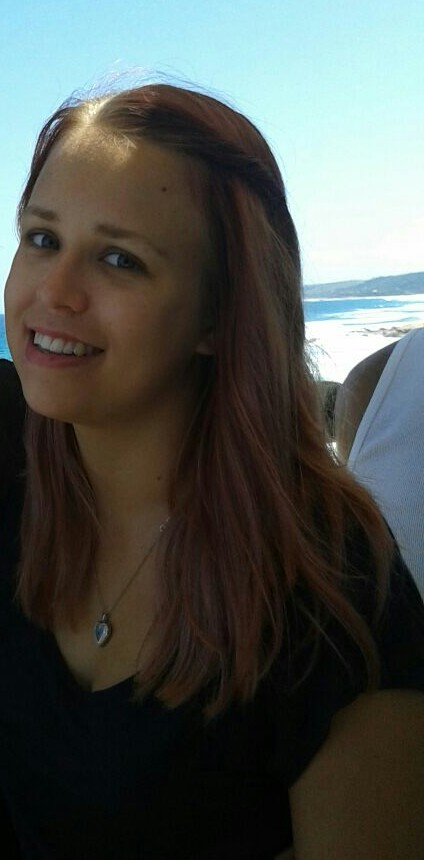
\includegraphics[height=0.3\textheight]{../Liz.jpg}
	\end{figure}
	\begin{itemize}
		\item \textbf{Full Name:} Elizabeth Fae Bode
		\item \textbf{My Interests:}
		\subitem Puzzle Games (eg. Sudoku)
		\subitem Computers
		\subitem Art
		\subitem Music
		\subitem User experience design
		\subitem Website design
		\subitem Gardening
		\subitem Reading books
		
		\item \textbf{My Technical Skills:}
		\subitem Web development skills
		\subitem Database design
		\subitem Java
		\subitem C\#
		\subitem C++
		\subitem Good at writing
		
		\item \textbf{Past Experience that Might Help:} \newline
		I have a decent accounting and mathematical background which should aid in the implementation of this project. I thoroughly enjoy web-development and interface design which is appropriate for this project as it is a necessary component that needs to be developed. I have dabbled in scraping components but I do not have much experience in scrapers nor do I have much experience in developing profiling engines. However, I am eager to learn both of these types of components and have no doubt that once I have an understanding of how to develop them, that I will be able to implement them with my team to the utmost of my ability.
		
		\item \textbf{Non-technical Strengths:}
		\subitem Good at decision-making
		\subitem Good at problem-solving
		\subitem Hardworking
		\subitem Organised
		\subitem Responsible
		\subitem Eager to learn new things
		\subitem Perfectionist
		
		\item \textbf{What makes me want to do this project?} \newline
		I am very interested in working with Retro Rabbit and have been since I spoke to a couple of their employees at the career day in the IT building at the University of Pretoria. I also enjoy, as mentioned above, web-development and have experience in both mathematics and accounting, which made me very interested in this project.
	\end{itemize}

		\subsection{C Saaiman}
	\begin{figure}[h]
		\centering
		
\includegraphics[height=0.3\textheight]{../Saaiman.jpg}
	\end{figure}
    
    \begin{itemize}
    \item \textbf{Full Name:} Christiaan Saaiman
    \item \textbf{My interests:}
    	\subitem Reading books
        \subitem Piano playing
        \subitem Gaming
        \subitem Coding
        \subitem Web Design
        \subitem User Experience Design
        \subitem Cooking and Baking
		\subitem Anime
        \subitem Languages
        	\subsubitem German
            \subsubitem Italian
            \subsubitem Japanese
        \subitem Artificial Intelligence
        \subitem Phones, Computer Hardware and Next-Gen Consoles

	\item \textbf{Technical Skills:}
    	\subitem Web Development Skills
        \subitem Java
        \subitem C++
        
	\item \textbf{Past experience:}
    	\subitem 6 Months intensive Java Training Course
        \subitem 6 Month Internship at Accenture
        	\subsubitem Intense Oracle Systems Training
            \subsubitem Leadership Training and meetings with the MD of Technology
            \subsubitem pitching an idea a colleague and I had.
            \subsubitem Tiger Brands' System upgrade from Oracle Database 11g to 12c
        \subitem Android App development using PhoneGap

    \item \textbf{Non-technical Strengths:}
    	\subitem Excellent Leader, not  afraid of conflict
        \subitem Excellent communicator
        \subitem Curious and eager to take on challenges
        \subitem Problem solver
        \subitem Dedicated and hardworking
        \subitem Creative and spontaneous
        
   \item \textbf{Reason for Project Tender:} \newline
   The project proposal peaked my interest in several ways. Firstly I thought the idea of creating and application that allows people to with ease and inexpensively generate an insurance risk profile was very very intriguing and exciting. It makes for a challenging and enticing problem that needs solving using creativity. Secondly I was also drawn to the technology usage. Not only is web development a necessary skill, but being able to write a Facebook Trawler, searching and gathering information is a whole challenge on its own. A very knowledge enriching challenge. Then lastly I am eager to learn from the experienced coders at Retro Rabbit. I would love to be able to delve into the rich information pools that will ultimately enable me to perform better.
	\end{itemize}
		
	\subsection{M Loosen}
	\begin{figure}[h]
		\centering
		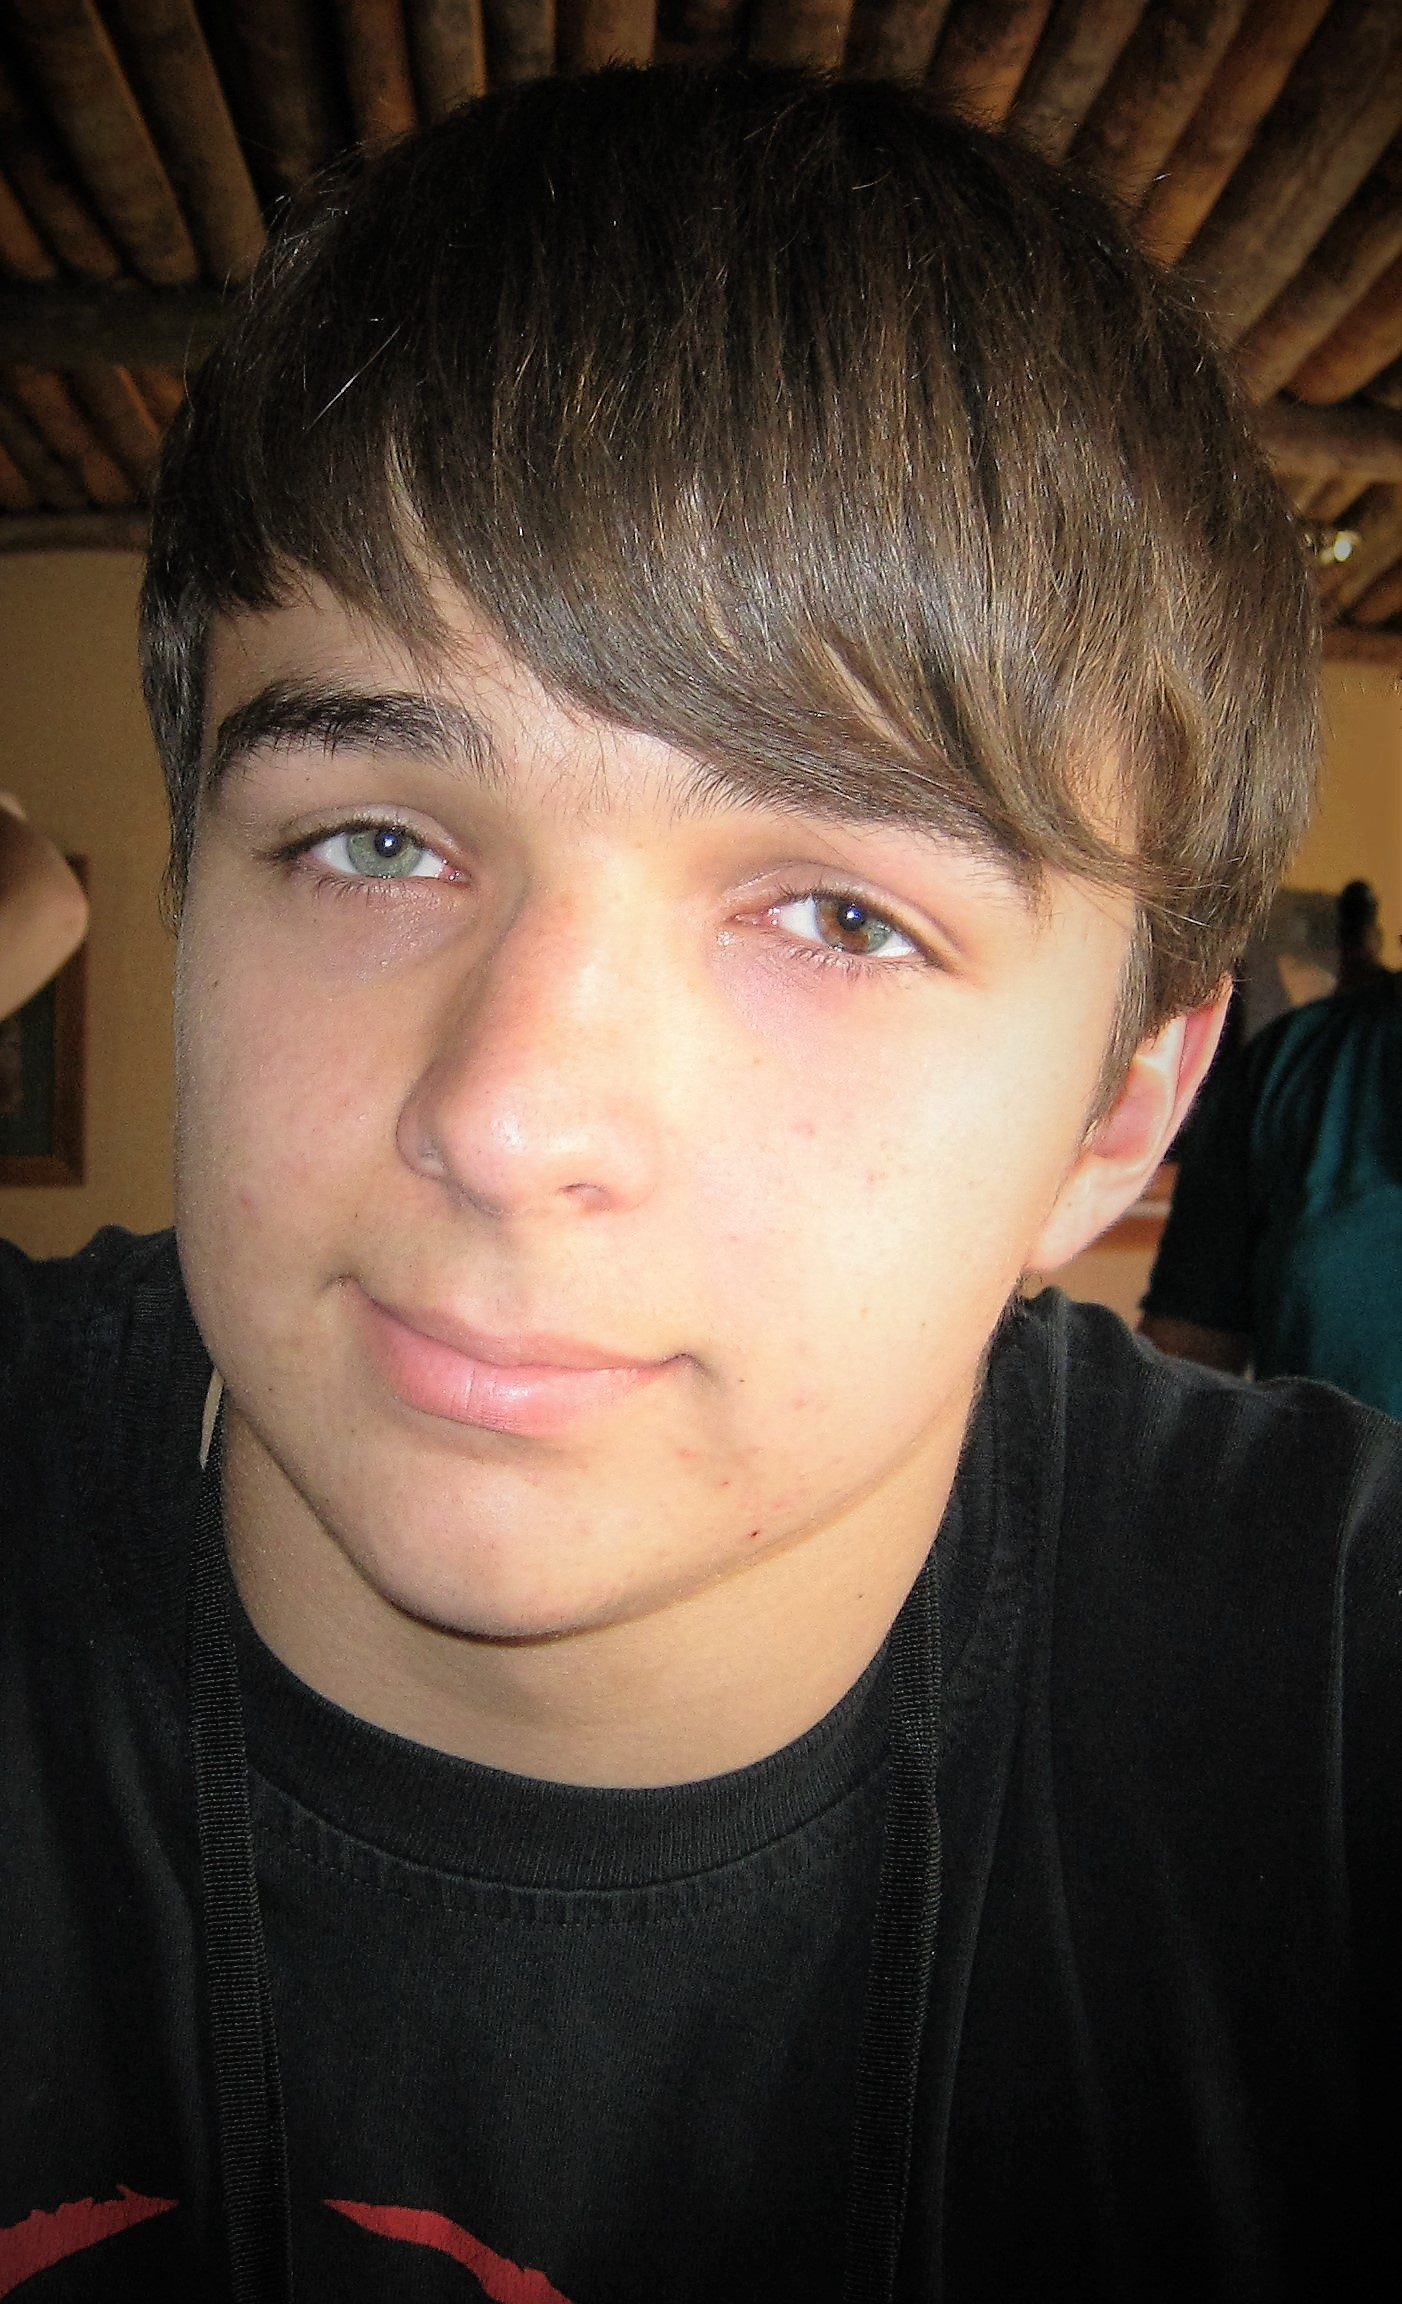
\includegraphics[height=0.3\textheight]{../Michael.jpg}
	\end{figure}
	\begin{itemize}
		\item \textbf{Full Name:} Michael Loosen
		\item \textbf{My Interests:}
		\subitem Gaming
		\subitem Coding
		\subitem Cooking
		\subitem Flying (Pilot)
		\subitem Motorcycles
		\subitem Planes
		\subitem Cars
		\subitem Music
		
		\item \textbf{My Technical Skills:}
		\subitem Database design
		\subitem Java development
		\subitem Web development skills		
		\subitem C\# development
		\subitem C++ development
		\subitem Technical document writing
		
		\item \textbf{Past Experience that Might Help:} \newline
		I have done accounting at school and also on varsity level, which I think might help in this project. My father, Dirk Loosen, has been in IT since before I was born and this is what lead to my interest in computers. I have learnt a lot from him, so I might have learnt something from him that could be of use. I also recently had the priveledge of job shadowing him at FNB Bank City. Here I was able to experience a large team of people working on a new application that was being developed using the Agile developement methodology.
		
		\item \textbf{Non-technical Strengths:}
		\subitem Good at problem solving
		\subitem Good at critical analysis
		\subitem Perfectionist		
		\subitem Good at decision making
		\subitem Hardworking
		\subitem Organised
		
		\item \textbf{What makes me want to do this project?} \newline
		When I read the project proposal I was intrigued by the idea of the project. I'm excited to work with Retro Rabbit as I think that I will enjoy it after reading up on the organization. I have a lot of accounting experience and enjoy mathematics, so when I saw what this project was about, I was excited to say the least.
	\end{itemize}
			
	\section{Project excecution}
	\begin{itemize}
		\item \textbf{Development Methodology} \newline \newline
		We plan to follow the Agile development methodology as it involves regular communication with the client to ensure the project results in exactly what they want. It also has a focus on the people system and their interactions with it which we believe is way more important than focusing on the processes and tools of the system. We strive to maintain a continues attention to designing the system well and ensuring that all the technical aspects are coherent with the requirements. All of which makes the Agile development methodology perfect for our vision for your project.
		
		\item \textbf{Progress Communication Plan} \newline \newline
		We plan on meeting up with you as the client on a regular basis, either face-to-face or via Skype, whichever is more convenient for you at the time, in order to keep you updated regarding the status of the project and to clarify requirements. We are also willing to communicate either via WhatsApp or email, whichever you prefer, in order to discuss the project and the progress of it, if face-to-face meetings are unable to take place for whatever reasons.

		\item \textbf{Technical Challenges \& Possible Solutions} \newline \newline
		We as a team believe we will have no problem with the front-end, as we are all well versed and experienced not only with Web Development but also User Experience Design. Our concerns lie with the Facebook scraper and the Profiling engine. We are not daunted by these two aspects of the project and we are very eager to learn the technologies needed for the project to be a success. We will be in close contact with Retro Rabbit and asking for assistance where we need it. Both Mr. Meyer as well as Mr. Saaiman is currently undergoing the Artificial Intelligence module at the university, so they will be able to apply their knowledge where necessary. As for Ms. Bode and Mr. Loosen, both are smart and hardworking and will not back down from unfamiliar waters. We will also consult with our other lecturers about the problems at hand if need be, especially Prof. Engelbrecht, our HOD.

		\item \textbf{Technologies we will use for the project:}
		\begin{itemize}
			\item For the front end we will use Bootstrap framework along with JQuery to handle AJAX requests to the server. Bootstrap makes making responsive websites very easy, thus the choice in Bootstrap.
			\item For the backend we will use Python along with Django. Django offers REST wrapping for the Ajax requests that will come from the client. Python is chosen because of the relative few lines of code for a task as opposed to Java. Therefore we will need less development time to develop a server with built in AI functionality to do the risk profiling.			
		\end{itemize}
		
		\item \textbf{What will be delivered to the client on project completion:} \newline \newline
		The aim is to produce a fully functional application that can allow users to insure their portable possessions. Our team will strive to produce this application to the best of our abbilities and will ensure that all of the required functionality is implemented correctly and that the application runs smoothly and is user friendly. The client will then receive this application and be able to use it to their benefit.
	\end{itemize}
\end{document}